\documentclass[dvipdfmx]{standalone}

\usepackage{tikz}

\begin{document}
\begin{tikzpicture}
    \node[anchor=west] at (-1,1) {50円硬貨までのみ使うなら、高々この額までであって欲しい。};

    \node at (0,0) {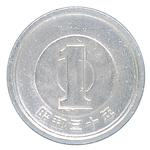
\includegraphics[width=1cm]{../imgs/yen/1.jpg}};
    \node at (1,0) {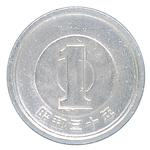
\includegraphics[width=1cm]{../imgs/yen/1.jpg}};
    \node at (2,0) {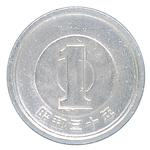
\includegraphics[width=1cm]{../imgs/yen/1.jpg}};
    \node at (3,0) {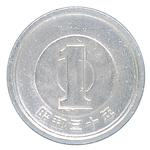
\includegraphics[width=1cm]{../imgs/yen/1.jpg}};
    \node at (4,0) {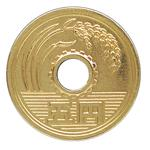
\includegraphics[width=1cm]{../imgs/yen/5.jpg}};
    \node at (5,0) {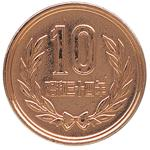
\includegraphics[width=1cm]{../imgs/yen/10.jpg}};
    \node at (6,0) {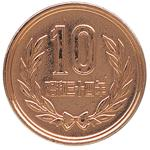
\includegraphics[width=1cm]{../imgs/yen/10.jpg}};
    \node at (7,0) {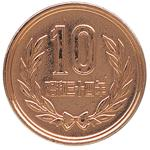
\includegraphics[width=1cm]{../imgs/yen/10.jpg}};
    \node at (8,0) {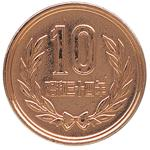
\includegraphics[width=1cm]{../imgs/yen/10.jpg}};
    \node at (9,0) {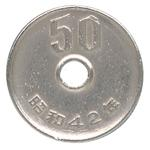
\includegraphics[width=1cm]{../imgs/yen/50.jpg}};
\end{tikzpicture}
\end{document}